\section{Introduction}
Recent years have seen advances in artificial intelligence conquer a number of problems that have, in the past, been very difficult to get at. These advances include text recognition \cite{GuRecentNetworks}, the besting of human play at the board game Go by Google's AlphaGo \cite{Silver2016MasteringSearch}, image classification \cite{GuRecentNetworks}, and even learning artistic style by example and applying it to images \cite{Gatys2015AStyle}. Recent advances in the field have been made by employing back-propagation with deep neural networks (networks with many hidden layers between the input and output layers). While this method is both powerful and computationally tractable, it has significant limitations including the necessity of supervised learning during the training process (each training input must be coupled with a known, desired output), poor ability to train networks with recurrence (i.e. networks with memory), the possibility of getting stuck at local maxima \cite[pg 312, 364]{Downing2015IntelligenceSystems}. 

Evolving Artificial Neural Networks (EANN) offers a network training mechanism with the potential to sidestep the aforementioned limitations of backpropagation training and, additionally, can be naturally extended to allow for online network adaptability \cite{Tonelli2013OnNetworks}. The potential of EANN to rival both the scale and plasticity of their biological counterparts is widely recognized \cite{Tonelli2013OnNetworks}; thus, EANN represent a route towards a more dynamic, general artificial intelligence. 

EANN methodology is centered on the evolutionary algorithm (EA), which --- inspired by biological evolution --- uses repeated evaluation, selection, and recombination of candidate solutions to evolve novel solutions to a wide array of problems. Researchers and engineers have widely demonstrated the ability of EA to provide good solutions to difficult optimization problems and to discover novel solutions beyond the reach of human ingenuity \cite{Poli2008AProgramming}.

Nonetheless, using EA to design artificial neural networks has proven a difficult task. In recent years, significant effort has been invested in studying and promoting evolvability, a term that although inconsistently and nebulously defined can generally be considered as the ability of the evolutionary process to generate useful variation in populations subjected to artificial evolution \cite{Richter2015EvolvabilitySurvey,Reisinger2005TowardsEvolvability, Wilder2015ReconcilingEvolvability}. Attempting to promote evolvability through traditional Darwinian fitness-based selection raises a conundrum: how is it possible to ``favor properties that may prove useful to a given lineage in the future, but have no present adaptive function'' \cite{Pigliucci2008IsEvolvable}? 

Indirect genetic encoding of candidate networks and the Baldwin effect have both been proposed as potential mechanisms to promote evolvability \cite{Reisinger2007AcquiringRepresentations,Downing2010TheNetworks}. Indirect genetic encoding has been demonstrated to produce an inherent bias towards phenotypic regularity in the evolutionary search space \cite{Tonelli2013OnNetworks} which enhances evolvability in problem domains with significant regularity, allowing the evolutionary algorithm to discover higher quality solutions than is possible with a direct encoding  \cite{Clune2011OnRegularity}. The bias of indirect genetic encoding towards phenotypic regularity is illustrated in Figure \ref{fig:indirect_bias}. While indirect genetic encoding creates regularity creates evolvability necessary to discover high quality solutions, in most problem domains the performance of a network generated by indirect encoding can be further enhanced by an irregular refinement, which has been likened to learning \cite{Clune2011OnRegularity}. In addition to improving the quality of individual solutions, it is thought that phenotypic plasticity --- in particular, learning --- might bias evolutionary search toward useful adaptation by incorporating information from local search of the fitness landscape into the fitness score of an individual; such local search effectively smooths the fitness landscape, making high fitness peaks more likely to be discovered and ``buying evolutionary time'' until heritable scaffolding to support the adaptation originally obtained via plasticity can be developed. This concept, illustrated in Figure \ref{fig:baldwin_effect}, is termed the Baldwin effect \cite{Downing2010TheNetworks,Downing2009ComputationalEffect}.

\begin{figure} 
   \centering
     \hfill
    \begin{subfigure}[b]{0.4\textwidth}
        \centering
        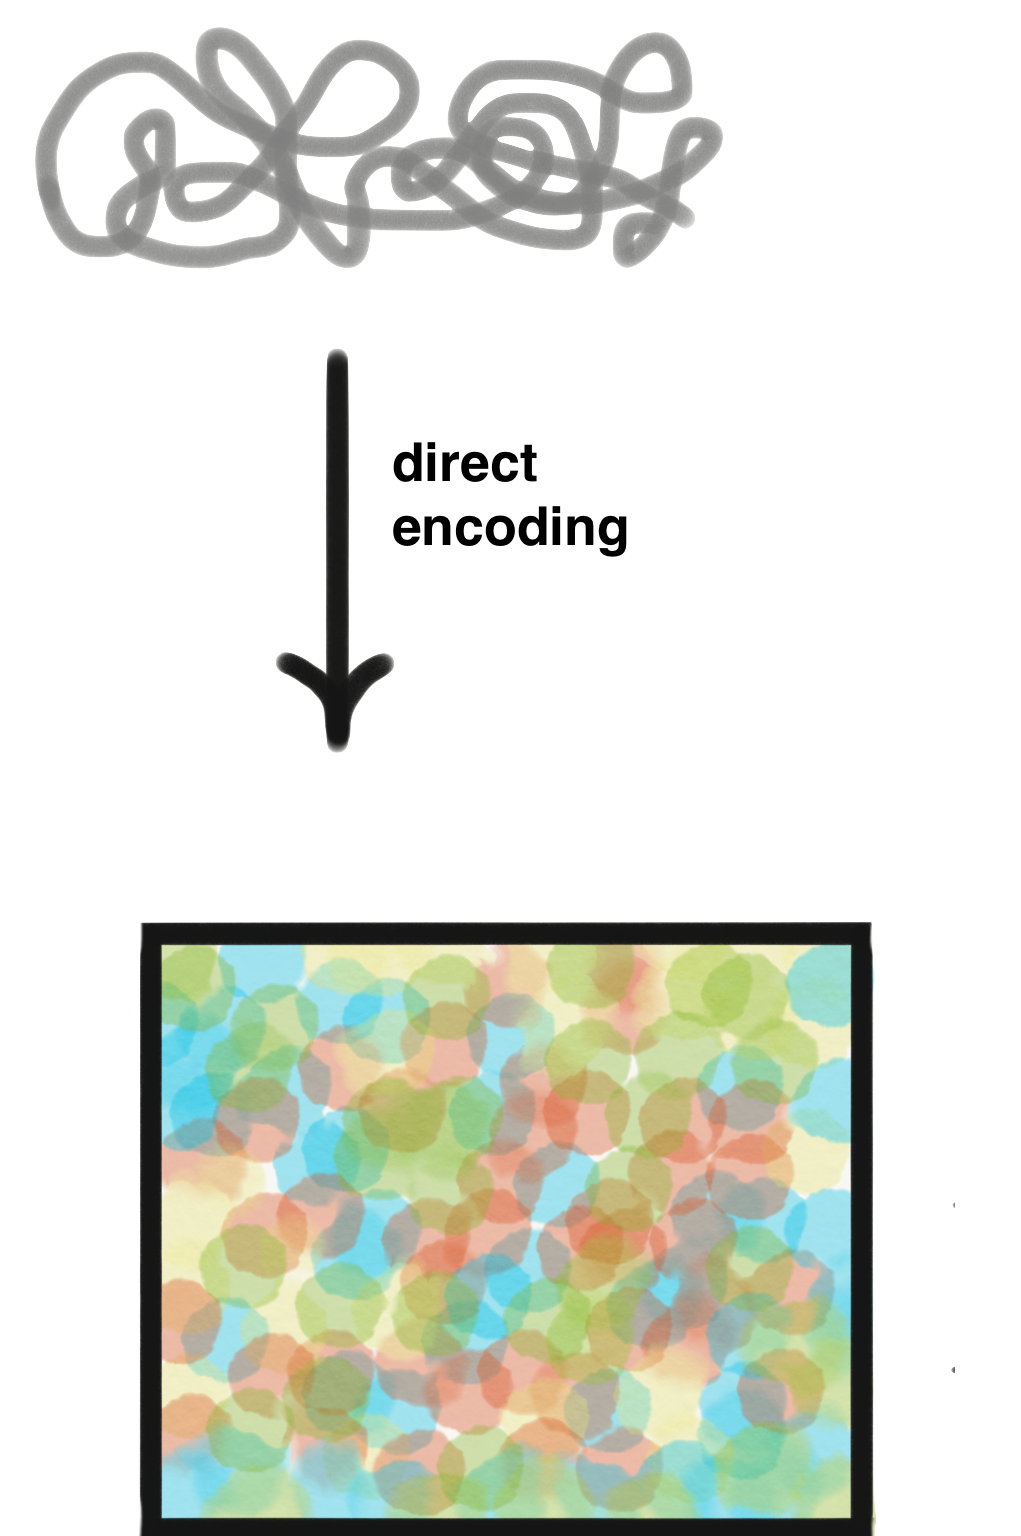
\includegraphics[width=\textwidth]{img/irregularity_direct_encoding.png}
        \caption{direct encoding}
        \label{subfig:direct_encoding}
    \end{subfigure}
    \hfill
    \begin{subfigure}[b]{0.4\textwidth}
        \centering
        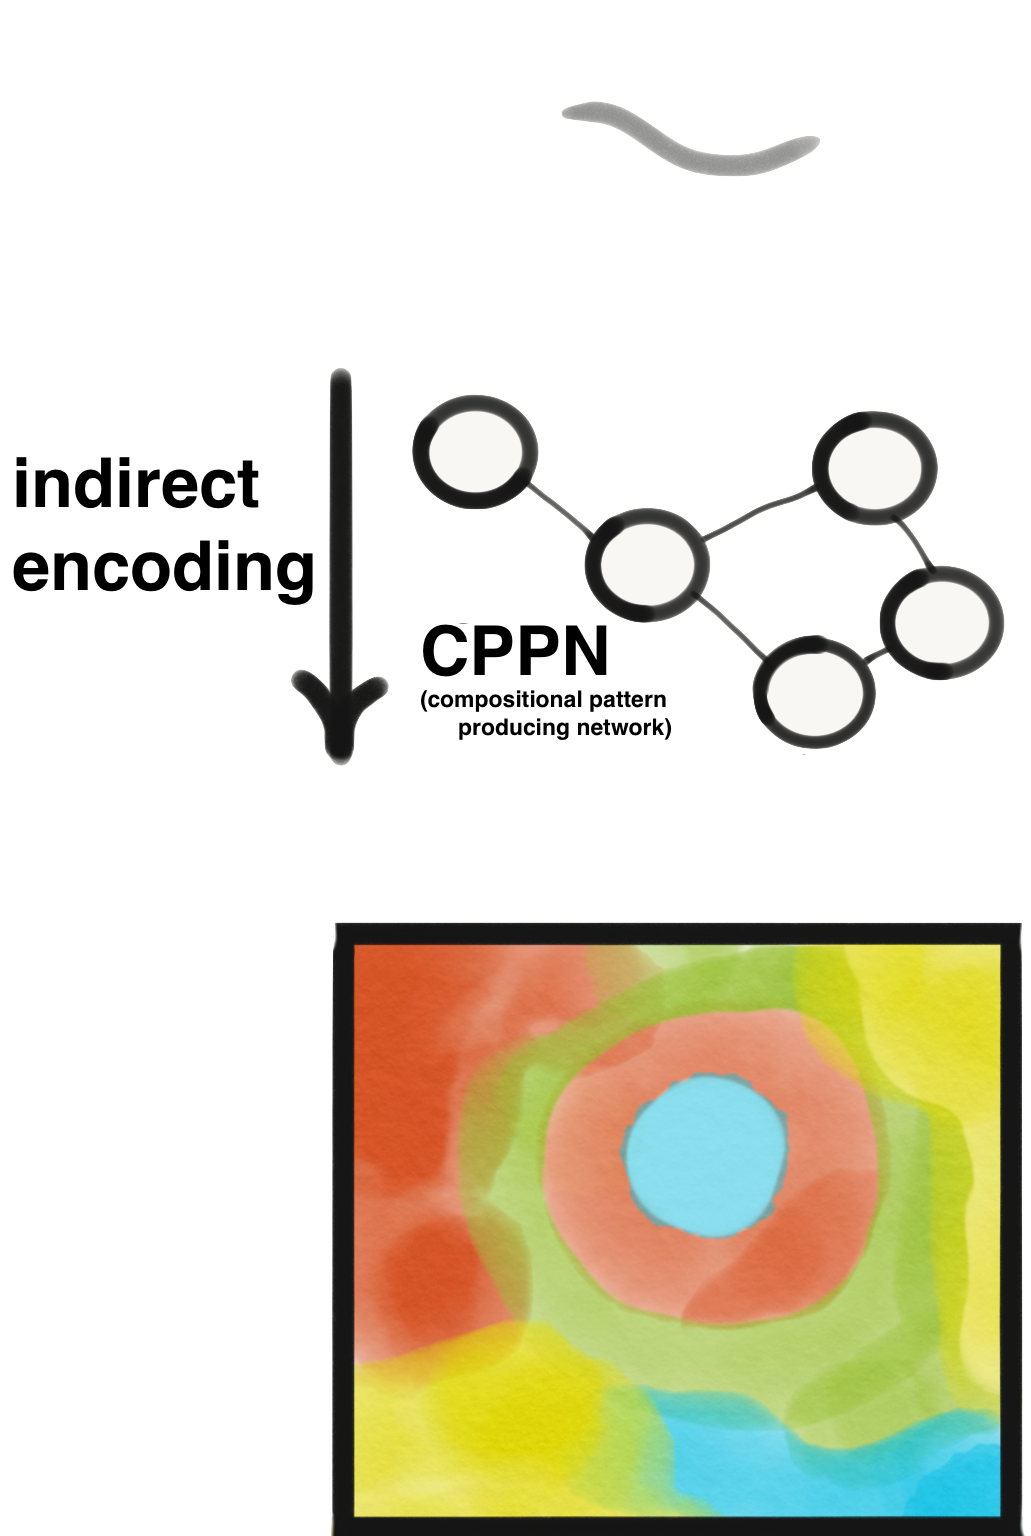
\includegraphics[width=\textwidth]{img/regular_indirect_encoding.png}
        \caption{indirect encoding}
        \label{subfig:indirect_encoding}
    \end{subfigure}
    \hfill
  \captionsetup{singlelinecheck=off,justification=raggedright}
  \caption{Archetypal examples of genotype to phenotype mapping from direct genetic representations and indirect phenotypic representations are illustrated. In both depictions, genetic information is shown at the top of the image and the corresponding phenotype is shown on the bottom of the image. In subfigure \ref{subfig:direct_encoding}, which depicts a direct encoding, a large volume of genetic information (where each characteristic of the phenotype is explicitly and independently described) is directly translated into a phenotype. Subfigure \ref{subfig:indirect_encoding} depicts an indirect encoding. In this particular scheme, a small amount of genetic information describes the configuration of a compositional pattern producing network (CPPN). This CPPN is then used to generate a phenotype. Indirect encodings are generally biased towards phenotypic regularity because phenotypic information is generated from a smaller amount of genetic information via a process that allows for multiple phenotypic elements to be determined by processes that tend to favor regularity and allows for genetic information to be reused to describe different components of the phenotype  \cite{Clune2011OnRegularity}.}
  \label{fig:indirect_bias}
\end{figure}

\begin{figure}
  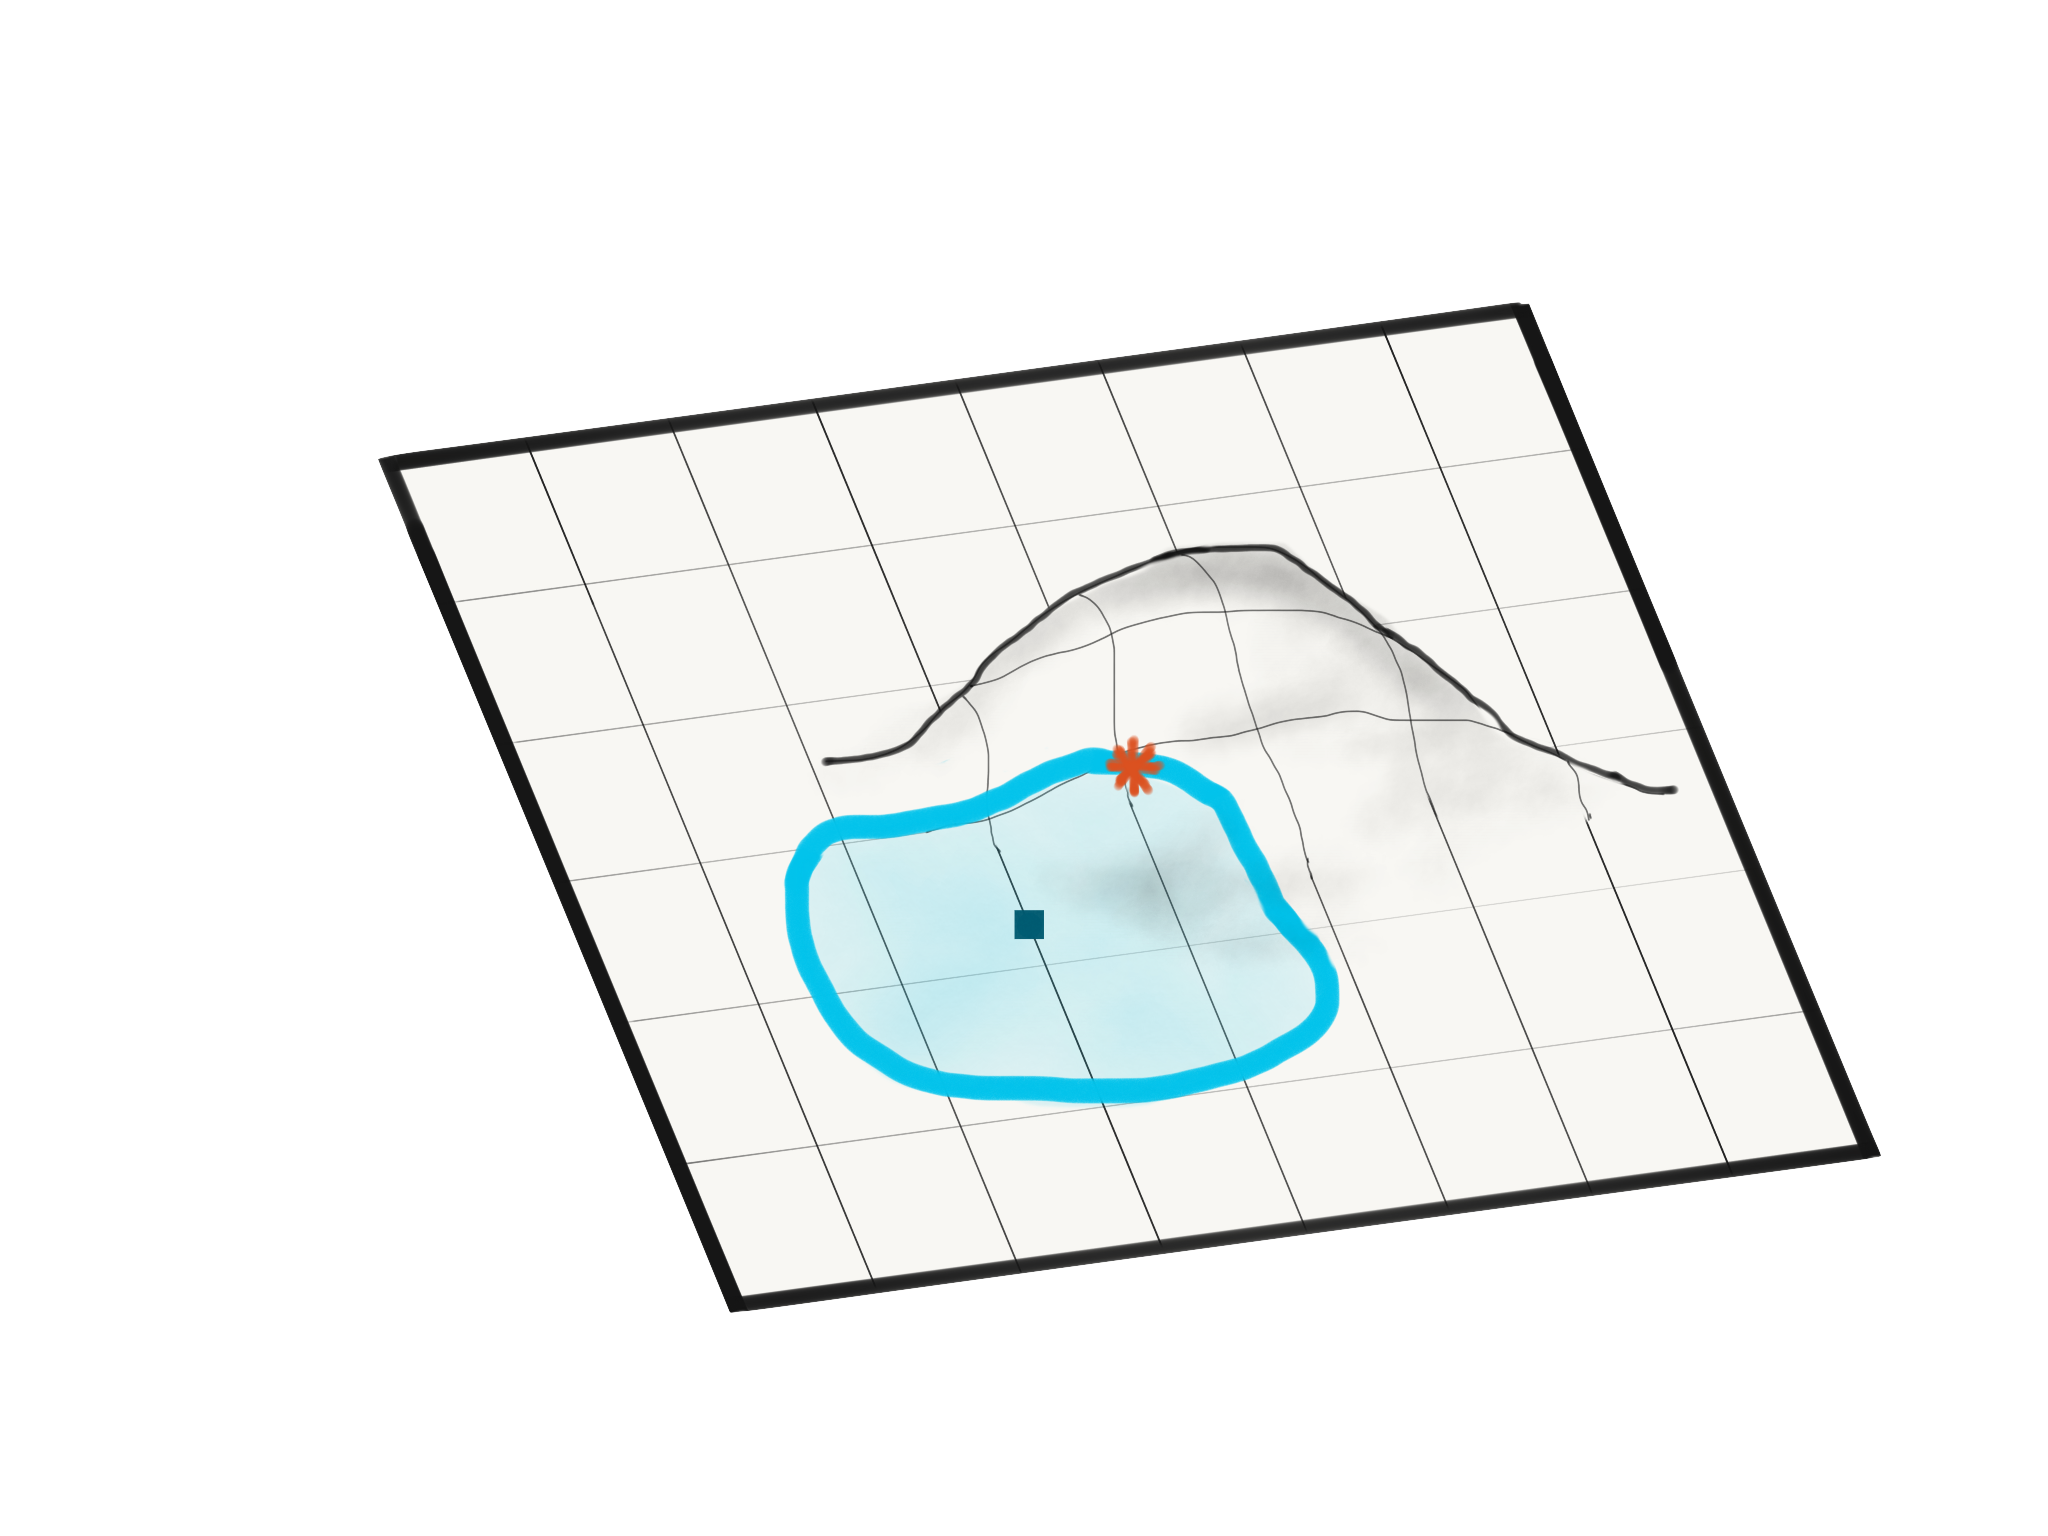
\includegraphics[width=0.8\textwidth]{img/baldwin_effect.png}
  \captionsetup{singlelinecheck=off,justification=raggedright}
  \caption{The Baldwin effect postulates that learning --- in evolutionary terms phenotypic plasticity or, equivalently and more explicitly, local search in the phenotype space --- biases evolutionary search to allow advantageous phenotypic features originally acquired via phenotypic plasticity to encoded into the genetic representation \cite{Downing2010TheNetworks}. In the first phase of the Baldwin effect, advantageous phenotypic features discovered by local search in the phenotype space increase the fitness of individuals proximal to that phenotype. Phenotypic plasticity is illustrated in the above cartoon, where the phenotype space is depicted as a three dimensional surface with points on the surface representing different phenotypes and the height of the surface denoting the fitness of the phenotypes at those points. In the illustration, the dark blue square represents the phenotype originally mapped to by the genetic representation of an individual, the blue shaded region represents the region of the phenotype space searched via phenotypic plasticity, and the red star represents a high fitness phenotypic variant reached via phenotypic plasticity. The fitness boost gained from phenotypic proximity to a high fitness solution biases evolutionary search to continue exploring that region of the instead of proceeding in other directions. In the second phase of the Baldwin effect, that continued evolutionary search promotes phenotypic features discovered by phenotypic plasticity are encoded into the genetic representation. Cost or unreliability of generating the advantageous phenotypic feature via phenotypic plasticity provides evolutionary pressure that favors genetic encoding of that phenotypic feature. In the case of indirect genotype to phenotype mappings, a direct genetic encoding of the feature discovered via phenotypic plasticity might not exist; however, genomes that map to phenotypes closer to the phenotypic feature discovered by plasticity --- which support attainment of the phenotypic feature by reducing the cost or increasing the reliability of acquiring that feature via plasticity, providing ``scaffolding'' for the local phenotypic search --- may still arise and will be selected for \cite{DowningHeterochronousBaldwinism}.}
     \label{fig:baldwin_effect}
\end{figure}

The development of methodology to promote discovery of neural architectures that, irrespective of prototypic fitness, have the potential generate networks that exhibit high fitness via irregular refinement. In other words, that serve as a platform on which direct-encoded evolutionary search, lifetime learning, or another irregular refinement technique can operate successfully. While research into the Baldwin effect has suggested that local phenotypic search can bias evolutionary search toward that provide scaffolding for phenotypic characteristics developed via local search, it not well understood what type of local search and what the minimal amount of it is that can bias evolutionary search towards solutions that have the potential to generate high performance solutions via irregular refinement. Because performing extensive irregular refinement to a candidate solution is computationally expensive, biasing evolutionary search towards neural architectures with high potential for enhancement via irregular refinement by explicitly computing the performance of the network after irregular refinement is not feasible. A less computationally expensive technique to estimate irregular refinement potential could improve the quality of solutions accessible via evolutionary search with indirect encodings and subsequent irregular refinement.

My research goal is to investigate how different methodology of phenotypic plasticity (local search) --- specifically, how local phenotypic exploration is organized and how fitness is computed based on the results of that local exploration --- to investigate what characteristics of phenotypic plasticity promote discovery of neural architectures with high potential for enhancement via irregular refinement. Restated, my research goal is to investigate the effectiveness of employing Monte Carlo methodology to explore the local phenotypic space of candidate neural architectures  at biasing evolutionary search towards the production of networks with high potential for enhancement via irregular refinement. In a series of experiments, local search will be performed via mutation to the direct-encoded representation of candidate neural architectures. Three variants of local search will be tested: simple mutation of the candidate neural architecture, mutational random walk from the candidate neural architecture, and simulated-annealing search. (Figure \ref{fig:local_search_types} illustrates these three modes of local phenotypic search). Additionally, three quantification schemes for the results of the local search will be considered: reporting of the 50th, 75th, and 100th percentile fitness scores of phenotypes encountered. It is hoped that considering these search and quantification schemes will shed light on what information about local phenotype space surrounding candidate solutions is necessary to bias evolutionary search towards neural architectures with high potential for enhancement via irregular refinement, ultimately providing a more complete picture of how phenotypic plasticity might promote the evolution of neural architectures capable of learning.

% , the capability to bias evolutionary search towards solutions , essentially to employ Monte Carlo methodology to estimate potential for enhancement via irregular refinement through  be nice to have a way to bias the evolutionary search while performing only minimal irregular refinement (local search) at each fitness evaluation.

% Monte Carlo

% Ultimately, the goal is to that can traverse the regular indirect genotype space but choose genotypes that have high fitness irregular regions around them that can be accessed via learning. How can we bias the evolutionary search to make this happen? How much information about the irregular regions around regular genotype mappings... what kind of search do we have to do to make sure that we end up somewhere with high potential to be enhanced via irregular refinement (learning).

% I wonder how incorporating information about the local space into fitness evaluation affects the amount of learning that is able to take place. The potential of the performance of a network to be enhanced by irregular modification.

% The role of irregularity here

% by incorporating information gleaned from local search in the fitness landscape into the fitness score of , thereby promoting evolvability.



% The idea is to create a regular base and then  \cite{Tonelli2013OnNetworks}

% ``suggest that HyperNEAT can benefit from a process of refinement that adjusts individual link patterns in an irregular way. While a direct encoding provides such refinement in this paper, there are other candidate refinement processes. One intriguing possibility is that lifetime adaptation via learning can play a similar role [44], [49]– [51]. Lifetime learning algorithms could adjust the overall regular patterns produced by HyperNEAT to account for necessary irregularities. Having a learning algorithm serve as the refining process may be superior to a direct encoding'' \cite{Clune2011OnRegularity}



 
% Bias towards regularity from i
 

 
% Tie together Baldwin effect and 

% Baldwin effect!!! plasticity in biology \cite{MoczekTheInnovation}.

% The concept of evolvability is a major focus of the field. Although there is no consensus for an exact definition of the term, evolvability is can be presented as the idea that properties beyond the immediate fitness of a solution are important to the success of the evolutionary process; a solution's potential to yield offspring of higher fitness must also be considered. Two main conceptions of evolvability have emerged: the ability to generate heritable variation \cite{Wilder2015ReconcilingEvolvability} and the ability to canalize mutations, biasing variation towards dimensions likely to be useful in the evolutionary search \cite{Reisinger2007AcquiringRepresentations}. 

% Attempts to promote evolvability generally fall into two categories: indirect encodings, where a developmental process maps between a compressed genotype and the phenotypic structure of a network, and selection pressure, where the rules for selecting members of the next generation are altered. Indirect encodings such as HyperNEAT are known to inherently bias the evolutionary search towards highly regular (i.e. symmetric) phenotypes, which is useful because most problem domains have a significant degree of regularity \cite{Clune2011OnRegularity} and because this regularity promotes ``spandrels'' in evolved solutions, which allows for more generalized learning abilities when learning rules are incorporated \cite{Tonelli2013OnNetworks}. Although most problem domains are highly regular, they do contain a degree of irregularity. It has been demonstrated that after a network is evolved indirect encoding, solutions can be further refined by allowing irregularity to be introduced via evolution with a direct encoding \cite{Clune2011OnRegularity}. The question of irregularity because networks that can be augmented by irregular search are potentially good candidates for post-developmental modification --- learning, an avenue to introduce irregularity to a network \cite{Clune2011OnRegularity}. It is currently thought that phenotypic plasticity in the form of learning can increase the 

% The goal of my project is to investigate the 
% The goal of my project is to investigate the relationship between a network's amenability to irregularization via direct search and local search in the phenotype space during the evolutionary process. The question is if sampling the local phenotypic space via irregularization will bias the evolutionary search towards regions of the search space that are more amenable by irregularization via FT-NEAT. In genetic regulatory networks, incorporating information about the local phenotype space of individuals leads to selection pressure for canalizing features in the genotype \cite{Reisinger2005TowardsEvolvability}. I plan to test this both in the context of post-evolutionary direct-encoded search.

% inspired by Baldwin effect and plasticity in biology

% amount to Monte Carlo sampling of the phenotypic space surrounding an individual

% Indirect encodings favor regularity ; selection pressure   favor regularity and allow for information beyond just the configuration of the network to be stored, and selection pressure.

% How can natural selection ``favor properties hat may prove useful to a given lineage in the future, but have no present adaptive function''? \cite{Pigliucci2008IsEvolvable}


% Evolvability is a central question... Indirect encodings generating selection pressure for evolvability.



% \begin{itemize}
% which offers the potential for online learning and more general artificial intelligence.
%   \item limitations in this technique include needing to do supervised training, -> an alternate paradigm!; also if we want a online learning and a more general artificial intelligence this is the way to go
%   \item If we want to get the Plasticity and scale of biological networks, we will need to evolve our way there
%   \item evolutionary algorithms are a well-established field, this is how they work
%   \item applying EA to artificial neural networks, indirect encodings such as hyperNEAT and selective pressure
%   \item indirect encodings bias towards regularity,
%   \item levels of search beyond just the naive evolutionary search (i.e. learning, development are both search processes) \cite{Downing2015IntelligenceSystems}
  
%   \item The goal of my research is to investigate the interplay between the evolutionary search and the learning search
%   \item look and see if incorporating local search as in \cite{Reisinger2005TowardsEvolvability} can affect the effectiveness of the FT-NEAT phase of HybrID (which is a stand-in for learning)
%   \item then, look and see if incorporating local search ... something... connect to Mouret \cite{Tonelli2013OnNetworks} (move on from direct representation addition of irregularity to addition of irregularity via learning)-
%   \item HybrID (hyperNEAT and FT-NEAT) \cite{Clune2011OnRegularity}, Baldwin effect [Downing], spandrels \cite{Tonelli2013OnNetworks}, Neural Darwinism \cite{Downing2015IntelligenceSystems}
  
% \end{itemize}